\chapter{Methods}
II. Methods
	A. Study Area
	B. Modeling Framework- RMLands (Kevin will write this)
	i. HRV
		1. Data prep
			B. Common Input Layers
				1. Input Layers: source, processing, purpose
		C. Model Parameterization
				1. State and Transition Models
				2. Disturbance parameters
					a. Climate
					b. Susceptibility
					c. Initiation
					d. Spread
					e. Mortality
		D. Model Calibration
		E. Model Execution
			3. Run parameters
				f. length/timesteps
		F. Data analysis
			1. Disturbance regime
			2. Vegetation response 
				a. Landscape composition (covcond plots)
				b. Landscape Structure/Patterns
	ii. Future Veg Treatments (match this to HRV header styles)
		1. Data prep
			B. Common Input Layers
				1. Input Layers: source, processing, purpose
		C. Model Parameterization
				1. State and Transition Models
				2. Disturbance parameters
					a. Climate
					b. Susceptibility
					c. Initiation
					d. Spread
					e. Mortality
		D. Model Calibration
		E. Model Execution
			3. Run parameters
				f. length/timesteps
			2. Post-processing (rescale, clip)
		F. Data analysis
			1. Disturbance regime
			2. Vegetation response 
				a. Landscape composition (covcond plots)
				b. Landscape Structure/Patterns

\section{Study Area}
\begin{figure}
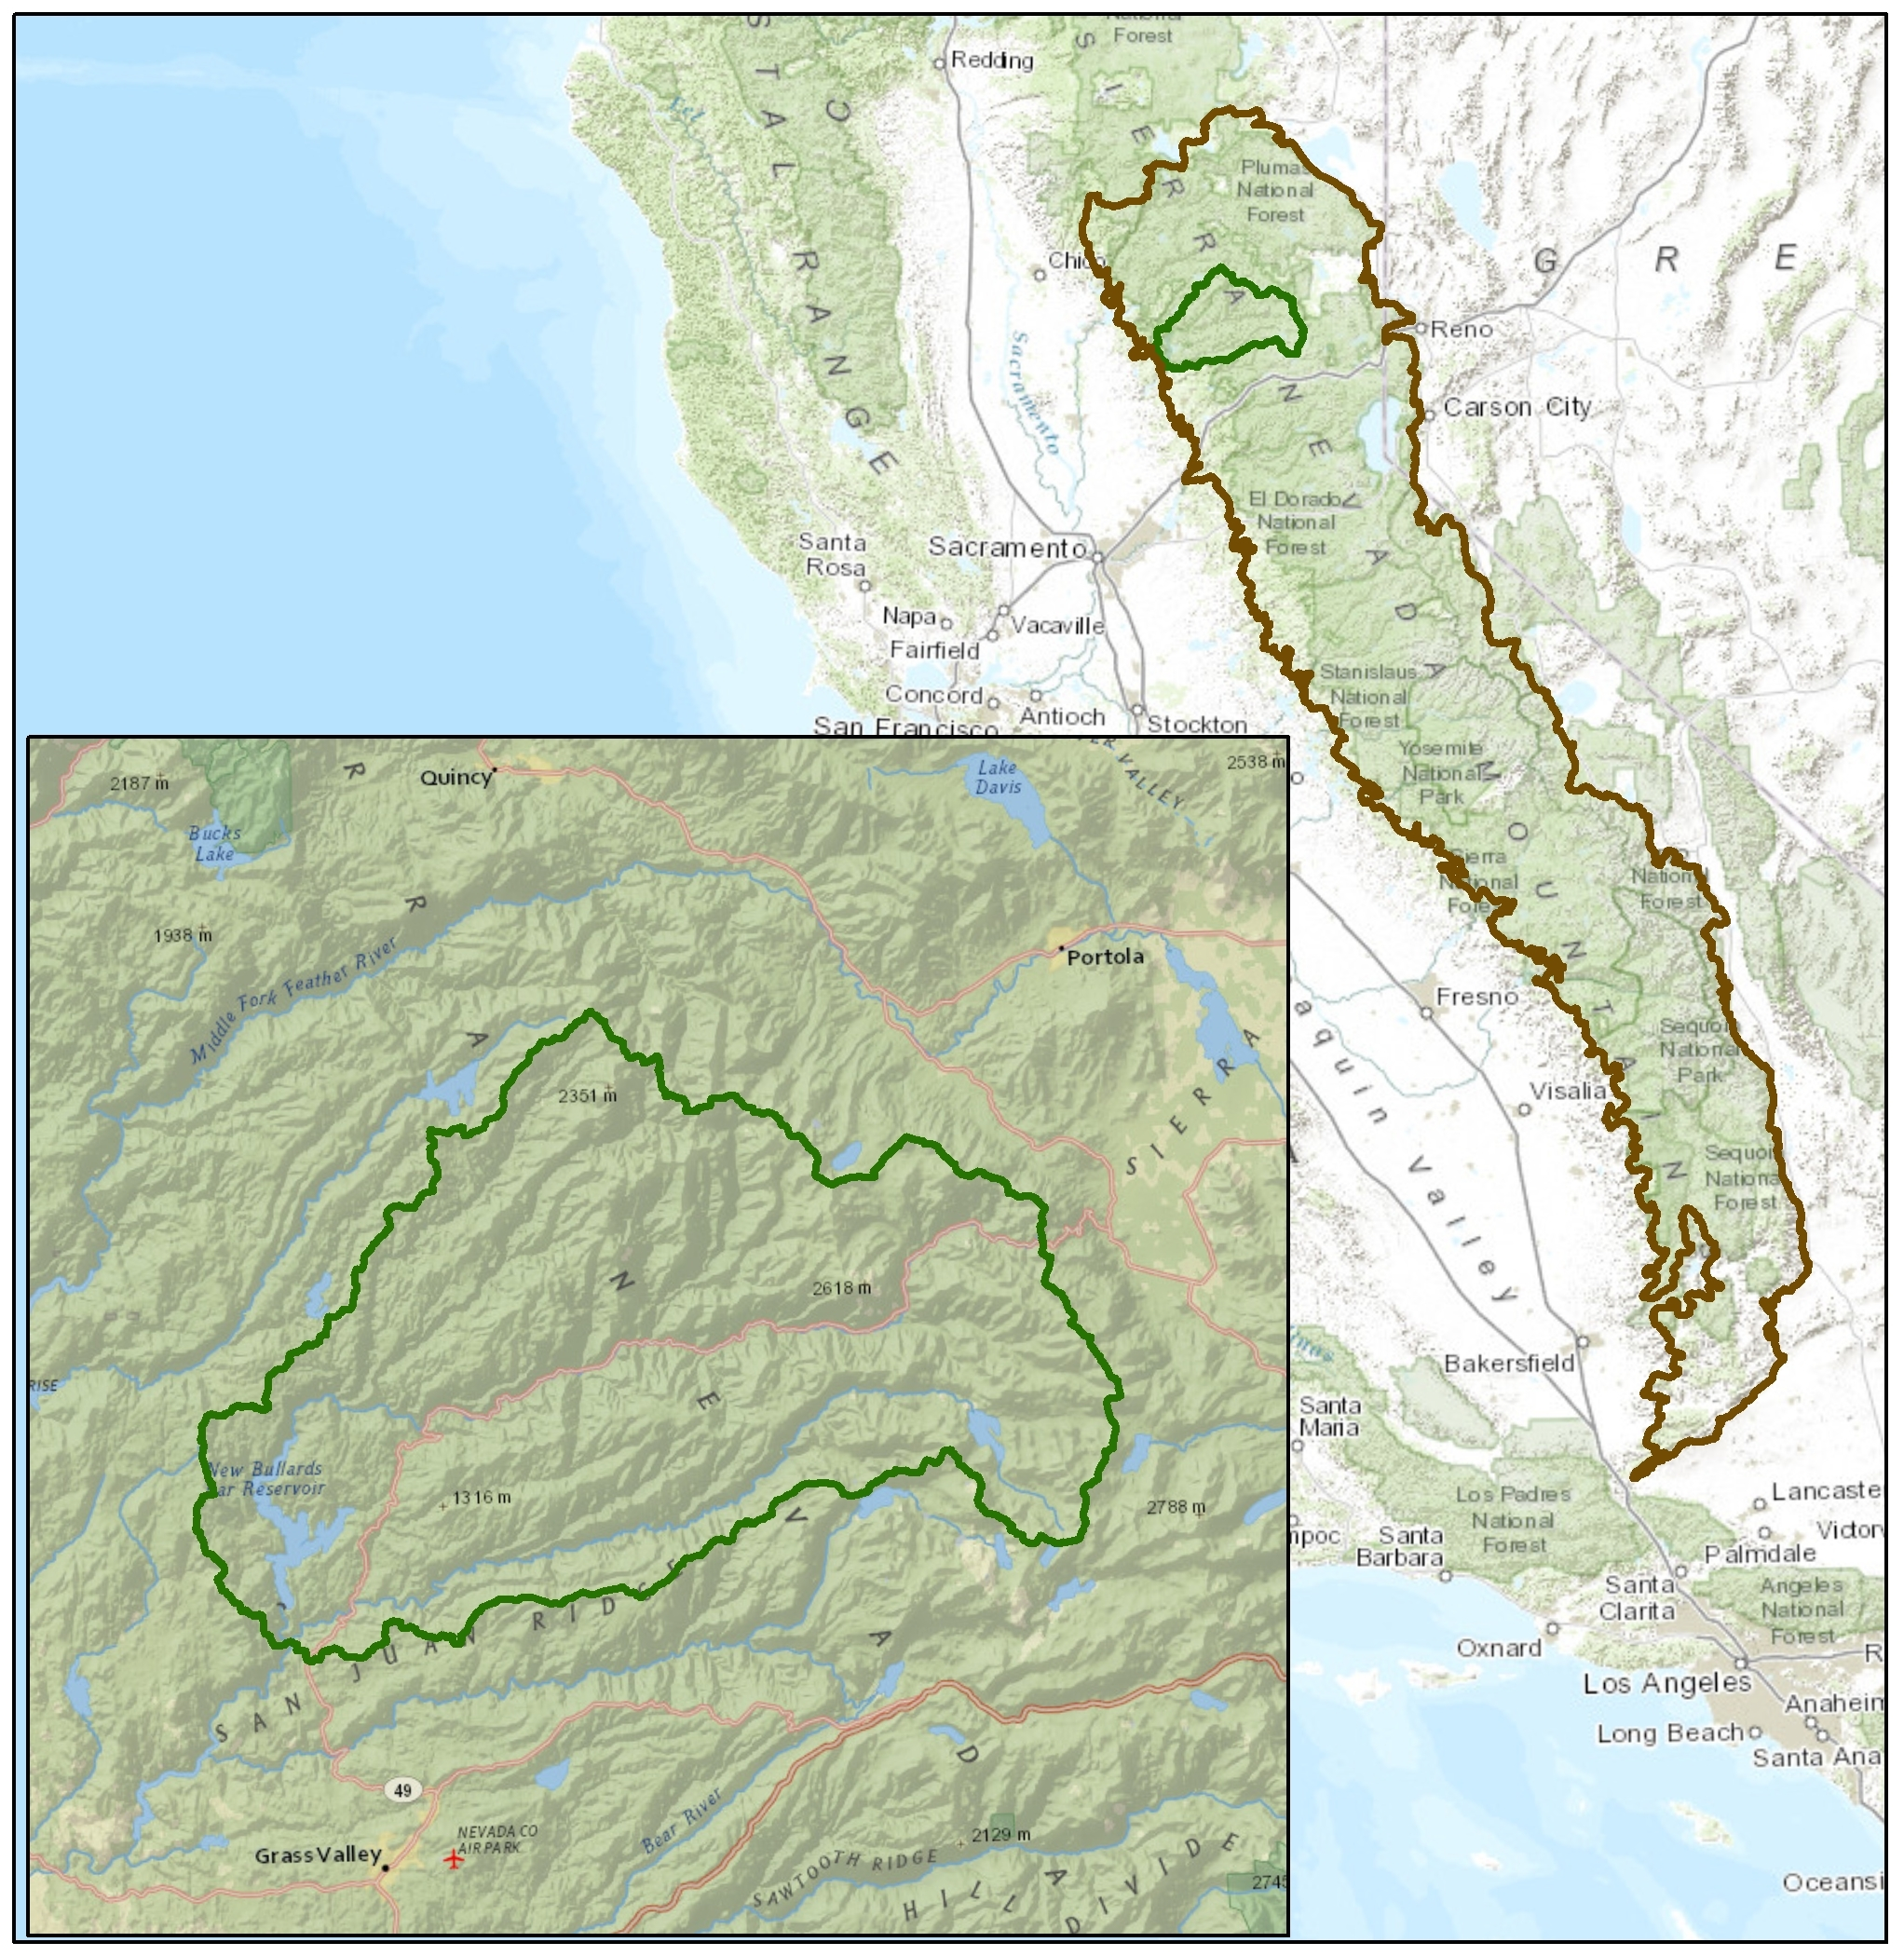
\includegraphics[]{ecoregionprojectarea.jpg}
\caption{The Sierra Nevada Ecoregion is highlighted in brown. The project landscape is located in the northern extent of the Sierra Nevada on the Tahoe National Forest, comprising the Yuba River watershed.}
\label{projectarea}
\end{figure}
The Sierra Nevada is a major North American mountain range, located east of California's Central Valley and extending from Fredonyer Pass in the north to southern Kern County in the south. Much of the Sierra Nevada is reserved as federally-held public land, managed by the U.S. Forest Service, Bureau of Land Management, and the National Park Service. The Plumas and Tahoe National Forests are located in the northern portion of the Sierra Nevada. The project landscape (see \ref{projectarea}) is located on the northern part of the Tahoe National Forest, on the Yuba River and Sierraville Ranger Districts, and comprises about 181,550 hectares. It is composed of a set of three HUC-5 watersheds, the Upper North Yuba River, the Middle Yuba River, and the Lower North Yuba River, referred to in this document as the Upper Yuba River watershed. 

The topography of the project landscape consists of rugged mountains incised by two major and a few minor river drainages. Elevation ranges from about 350 to 2500 meters. The area receives 30-260 cm of precipitation annually, most of which falls as snow in the mid to upper elevations (Storer and Usinger 1963). Some areas in the mid-elevation band receive high precipitation compared to the region, resulting in patches of exceptionally productive forest (Alan Doerr, pers. comm.). Vegetation is tremendously diverse and changes slowly along an elevational gradient and in response to local changes in drainage, aspect, and soil structure. Grasslands, chaparral, oak woodlands, mixed conifer forests, and subalpine forests are all found within the study area. Many species exhibit fire-adapted traits, such as resprouting from roots post-fire (e.g. tanoak), fire-induced germination (e.g. manzanita), or thick bark (e.g. ponderosa pine). 

Prior to European settlement, wildfire was a major source of disturbance on the landscape, shaping the composition and configuration of vegetation in the Forest. Fires were primarily lightning-caused, although indigenous peoples are thought to have set fires for vegetation management, especially in the lower elevations. In general, fire was frequent, with a mean rotation as short as 20 years in Ponderosa Pine dominated forests. Wetter mixed conifer areas are predicted to have had a mean fire rotation of 30 years. Fire rotation is thought to increase gradually with elevation, and mesic Red Fir had a mean fire rotation of 60 years. Variance around these means can be significant, as some parts of the forest experience fire much more frequently, while other escape fire for long periods. In general, regardless of vegetation type, high mortality fires were thought to be rare, with the vast majority of fires killing under 70\% of overstory trees. Under this disturbance regime, stand-replacing fire initiated early development conditions on the landscape. Low mortality fire tended to open forest canopies, while vegetation succession closed them again. The rarity of high mortality fire allowed large forest stands to succeed into late development and old growth conditions.

fire maintained open canopies in more xeric parts of the forest, while closed canopies were more persistent on more mesic, north and east-facing slopes. 

The arrival of Europeans in the 1850s sparked a transformation of this landscape as people harvested timber, extracted gold using hydraulic mining techniques, and suppressed wildfires (Storer and Usinger 1963). Forestry, mining, grazing, and dozens of recreational activities, including hunting, mountain biking, and hiking continue to take place on the Tahoe National Forest. Fifteen allotments exist within the project area for both cattle and sheep grazing. In addition, 231,368 hectares inside of the project area have non-Forest Service ownership. Many of these lands were privately held, often by timber companies, before the Forest was created. In addition, many public lands were given to the Central Pacific Railroad in the late 19th century, and this ``checkerboard'' ownership pattern persists today ADD FIGURE HERE. Mining of gold and other minerals also continues. These activities affect and interact with ongoing vegetation succession and disturbance processes in the area.

The Tahoe National Forest has an active fire management program, and maintains a cooperative agreement with the State of California to help fight wildfires on the non-Forest Service lands located with the Forest boundary. In the recent history of the forest, very few acres have burned, with the exception of 1960, when approximately 100,000 acres burned on the Forest. The low burned acreage corresponds with fairly high fire starts (both human- and lightning-caused) [Forest Plan]. Fire suppression has lead to an increase in the amount of dead and downed fuels in the forest (SNFramework).

Logging has been a major human impact on the Forest since European settlement. Clearcutting, shelterwood, salvage cutting, and plantation management have been major components of timber management on the TNF for several decades. More recently, group cut strategies replaced clearcutting as a management alternative. Together with fire suppression, timber management on the Forest has effected changes in forest composition. In general, shade intolerant species such as ponderosa pine, sugar pine, and Douglas fir have become less common, while shade tolderant species, especially white fir, have become more predominant [1990 Forest Plan]. In the last 20 years, timber sales in the Sierra Nevada have dropped drastically, but on the Tahoe National Forests timber sale levels have fluctuated both up and down (although annual sawtimber sold has decreased similarly to other Sierran Forests).


\section{Modeling Framework}

\section{Historic Range of Variability}

\paragraph{Data Structure} RMLANDS uses raster GeoTiffs (.tif files) as its data structure. Rasters are based on uniform square units called cells (or pixels). Each cell represents an actual portion of geographic space, where each cell has a defined X and Y value that corresponds to the coordinates defined by the projection. For example, in the Universal Transverse Mercator (UTM) projection, the grid that covers the entire Tahoe and Plumas National Forests project area is in UTM zone 10 N and covers an area defined by a range of X and Y values (minimum and maximum). In the Yuba River watershed landscape, each grid cell is 30 meters on a side (i.e., 900 m2 or 0.09 ha), and the input grid measures 2910 by 2245 pixels. All grids must be single-attribute, signed integer grids. Each cell is assigned a single class value, where valid class values are positive or negative whole numbers. All grids are created in ArcMap and saved as GeoTitff files before being input to the model. 

\paragraph{Raster layer alignment} RMLANDS requires that all grids are perfectly aligned. This means that not only must all grids have the same cell size and the same numbers of rows and columns, but the cells need to occupy the exact same geographic space (out to six decimal places) and have the same number of total cells. RMLands requires that all input grids are perfectly aligned. We accomplished this by setting the Extent and Snap Raster to the same parameters whenever we manipulated the layers in ArcMap. This ``base'' spatial layer was created by taking the primary elevation layer used on the Tahoe National Forest, resampling it to a 30 meter grid, and clipping its extent to match that of the buffered project area (2910 x 2245 grid size).

The input layers are: cover, condition, age, aspect, slope, elevation, streams, roads, and condition-age.

\subsection{Cover}
The \emph{cover} layer represents land cover type, which is often but not always the vegetation type (i.e. cover types include not only Lodgepole Pine, but also Barren, and Agriculture). The \emph{cover} does not change over time, and is used to define potential disturbance and succession transitions undergone by cells within a particular cover type.

Cover represents land cover type. Typically, cover type is based on the potential or current natural vegetation of a site and may include both natural and anthropogenic cover types. For example, cover types include not only Lodgepole Pine, Sierran Mixed Conifer, and Red Fir, but also Barren and Agriculture. Cover affects virtually every process in RMLANDS. Succession pathways are defined uniquely for each cover type, susceptibility to natural disturbances varies among cover types, and suitability or eligibility for various vegetation treatments varies among cover types. Cover is a ``static'' grid. Specifically, cover provides a fixed template upon which disturbance and succession processes play out over time. The cover type of a cell does not change over time; it is constant. All cells within the project boundary must be assigned a cover type; i.e., there can be no missing data or “background” within the project boundary. NODATA is reserved for all cells outside the project boundary.

The source for the cover layer is the Region 5 Existing Vegetation Layer, mapped to the CALVEG classification developed by the Region's Ecology Program in 1978. The CALVEG types in the project area are specific to the North Sierra mapping Zone. Within the project area, the Existing Vegetation Layer was developed based on three separate efforts: a satellite-based imagery analysis in 2000, and two orthoimagery analysis completed by contracting firms in 2005. Generally, specific cover type names were derived from the California Fire Return Interval Departure (FRID) report by Safford et al. (YEAR).

Geoprocessing for this layer was complex. Beyond converting the vector data to a raster format, further analysis was required to distinguish east- and west-side areas from one another, and generate the cover type modifications that the team agreed on. Aspen types were created by overlaying an aspen layer onto the vegetation layer and creating combined types (``type-aspen'')where appropriate. Areas mapped as a vegetation type characteristic of early seral (e.g. chaparral) were analyzed and assigned an appropriate forested cover type. Ultramafic types were created by overlaying a geology layer onto the vegetation layer and performing a similar processing step to create ``type-ultramafic''. Finally, for the Sierran Mixed Conifer and Red Fir cover types, which cover broad swaths of land across elevation and aspect, a xeric to mesic gradient was developed in conjunction with local experts and applied, creating ``type-mesic'' and ``type-xeric''.

Ultimately, 31 cover types were generated for the buffered project area:
\begin{verbatim}
YHR	Count	Landcover3
1	60173	AGR
2	97233	BAR
3	454		CMM
4	51302	GRASS
5	31289	LPN
6	349		LPN_ASP
7	50		LSG
8	38171	MED
9	150520	MEG_M
10	18388	MEG_U
11	153011	MEG_X
12	24627	MRIP
13	46514	OAK
14	632677	OCFW
15	24275	OCFW_U
16	381		RFR_ASP
17	218070	RFR_M
18	3564	RFR_U
19	110989	RFR_X
20	17773	SAGE
21	139365	SCN
22	69		SCN_ASP
23	1341	SMC_ASP
24	1488003	SMC_M
25	108605	SMC_U
26	1016037	SMC_X
27	8693	URB
28	91245	WAT
29	5668	WWP
30 	116653	YPN
31	34		YPN_ASP
\end{verbatim}

A thorough description of geoprocessing steps necessary to recreate this data layer are available HERE.

\subsection{condition}
Condition (or stand condition) represents the structural condition of vegetation for cover types that undergo succession. They represent discrete seral stages of stand development - as identified by experts, which may vary considerably among cover types. Condition can be used to affect virtually every process in RMLANDS. In particular, transitions among condition classes during stand development define the succession pathways for each cover type. In addition, condition can be specified as a factor affecting susceptibility to natural disturbances and suitability (or eligibility) for vegetation treatments. Condition is a “dynamic” grid; cell values change over time during the simulation in response to disturbance and succession processes. Ultimately, the combination of condition and cover defines the categorical classification of the landscape that provides the framework for characterizing vegetation patterns and dynamics.

All cells within the project boundary are assigned a condition class; i.e., there is no missing data or ``background'' within the project boundary. However, some cover types (e.g., roads, urban, agriculture, barren, water, mountain grassland, etc.) may not have multiple condition classes and can be assigned a common value. In addition, all condition classes do not need to exist for each cover type. 

The source for the condition layer is the Region 5 Existing Vegetation Layer, mapped to the CALVEG classification developed by the Region's Ecology Program in 1978. Within the project area, the Existing Vegetation Layer was developed based on three separate efforts: a satellite-based imagery analysis in 2000, and two orthoimagery analysis completed by contracting firms in 2005. All members of the team discussed potential attributes to be used for this classification, and identified attributes for tree diameter at breast height (DBH) and cover from above (CFA) to classify pixels into early, middle, or late development, and open, moderate, and closed canopy. In this application, aspen and shrub types have condition classes that differ from that of the remaining forest types. The other forested types use a consistent set of condition classes.

Geoprocessing for this layer was complex. Beyond converting the vector data to a raster format, further analysis was required to update the layer to a year 2010 condition. Spatial data on wildfire and timber management history was used to provide a more accurate assessment of condition based on estimated stand age. In addition, areas currently mapped as chaparral in the Existing Vegetation Layer were assigned to the early development stage.

\begin{verbatim}
Code	Count_	Condition
0		312508	Non-Seral
10		469764	Early All
20		790472	Mid Closed
21		919861	Mid Moderate
22		783077	Mid Open
30		598140	Late Closed
31		525793	Late Moderate
32		147522	Late Open
40		8		Early Aspen
41		380		Mid Aspen
42		1412	Mid Aspen Conifer
43		92		Late Conifer Aspen
\end{verbatim}

\subsection{Age}
Age represents the number of years since stand origin (i.e., the number of years since the last
stand-replacing disturbance), not necessarily the age of the oldest plant individuals in the stand. In some circumstances the age since stand origin can greatly exceed the age of the oldest individual plants (e.g., old-growth stands). Age can be derived in any manner. Typically, however, it is estimated in the field by direct observation or estimated through a process of interpolation based on ecological and/or geographic distance to stands with known age. Age affects a variety of processes in RMLANDS, including succession transitions and susceptibility to disturbance. Age is a ``dynamic'' grid; cell values change over time during the simulation in response to disturbance and succession processes.

Age values can be any positive whole number, although any precision less than the length of the model time step (5 years) is inconsequential. A “no age” value (99998) is assigned to all non-vegetated and non-seral cover types.

It is important to note that while age is potentially an important variable in RMLANDS——for example, it is typically the principal factor influencing succession transitions and can provide a basis for summarizing the range of variability in vegetation conditions––the ``initial'' age condition is a transient state that gets modified quickly during the simulation in response to disturbance and successsion processes. Therefore, the initial age structure of the landscape may be of little importance in a long-term simulation, as long as the model equilibration period (i.e., the period it takes the age structure of the landscape to stabilize given the disturbance regime) is properly accounted for.

In this application, we used data from stand exams dating to the 1960s and recent Ecology group survey plots to estimate stand age across the buffered project area. We then interpolated that information across the landscape. Due to insufficient data, we were unable to disaggregate the data below the landscape scale. We also acknowledge that the stand exam and modern veg plots do not constitute a true sample and were conducted almost exclusively in mid-mature and mature stands of commercially viable trees, thus skewing the results to some unquantifiable degree.

We updated the interpolated data with wildfire and timber management history, and assigned ages to types coded as chaparral in the Existing Vegetation layer to the midpoint of the age spread of early development for the forest cover type to which it was converted. Remaining ages out of compliance with allowed ages for the corresponding condition of a given cell were modified to be in compliance, based on the assumption that the condition class assignment was more accurate that the interpolated age information.

\subsection{Condition-Age}
Condition-Age represents the age since transitioning to the current condition. After creating both the condition and age layers, we used a Python function to derive condition-age based on the youngest possible age for a cell of that cover and condition. For example, if a pixel is Lodgepole Pine, Mid Development Closed, and 50 years old, we take the minimum age for that cover-condition combination (10 years old), and subtract it from the current to arrive at a condition-age of 40. 

\subsection{Topographic Position Index}
Our topographic position index combines slope position with heat load (itself based on aspect and slope). High values for TPI represent locations on upper slopes, tending toward south and west-facing aspects, and are relatively steep. Low values represent locations in valley bottoms, tending toward north and east-facing aspects, and are more gentle in slope. Values around zero represent locations tending towards the center of these extremes. We use TPI to adjust vegetation susceptibility and mortality because we expect susceptibility and mortality to be higher when TPI is high.

\subsection{Elevation} 
Elevation represents the height above sea level in meters. Elevation is typically derived from an existing digital elevation model (DEM). Elevation can be used to affect a variety of processes in RMLands, including succession transitions and susceptibility to disturbance. Elevation is a ``static'' grid; cell values remain constant over time. All cells within the project boundary must contain a real value; there can be no missing data (or nodata) cells. The elevation grid used in this analysis was provided by the Tahoe National Forest GIS staff and rescaled from 10m pixels.

\subsection{Slope} 
Slope represents the steepness of a cell as measured in percent. Slope is derived from elevation. Slope is used to affect a variety of processes in RMLands, including succession transitions, disturbance severity and eligibility for various vegetation treatments. Slope is a ``static'' grid; cell values remain constant over time. All cells within the project boundary contain a real value; there are no missing data (or nodata) cells. 

\subsection{Aspect} Aspect represents the direction that a cell faces. Aspect is derived from elevation. Aspect can be used to affect a variety of processes in RMLands, including succession transitions and disturbance susceptibility and severity. Aspect is a ``static'' grid; cell values remain constant over time. Grid values represent categorical values assigned to the eight cardinal directions, plus a value for flat areas with no aspect. All cells within the project boundary  contain a real value; there are no missing data (or nodata) cells. 

\subsection{Streams} 
Streams represents aquatic communities classified as small, medium or large based on
stream order. In this application, the streams layer was created from a line coverage containing hydrography data, including an attribute for stream size or order, by converting to a grid based on the stream size attribute. Streams are used to affect disturbance spread in RMLANDS; i.e., streams function as an impediment to spread. 

We employed the orthogonal neighbor rule when converting a line to a raster of like-valued cells. That is, the final grid contains stream cells that connect along a cell side, as opposed to diagonally. This is required because diagonal neighbors, while touching, will not provide an impediment to disturbance spread (which happens diagonally as well as orthogonally). In addition, streams do not have to be in a contiguous network (i.e., no breaks in the streams) as long as the implications in terms of disturbance spread and/or logical treatment boundaries are acceptable. 

Streams is a ``static'' grid; cell values remain constant over time. Note, streams are integrated into the cover type classification scheme only insofar as they are classified as type 'Water' in the Existing Vegetation Layer. Regardless, they also exist as a single layer. Grid values represent categorical values assigned to the three stream size classes, plus a value for background. All non-stream cells within the project boundary must be assigned a background value. NODATA is reserved for cells outside the project boundary. 

\subsection{Roads} 
Roads represents all transportation corridors classified as small, medium or large based on road size and/or intensity of use. 

In this application, the roads layer was created from a line coverage containing transportation data, including an attribute for roads size or order, by converting to a grid based on the roads size attribute. Roads are used to affect disturbance spread in RMLANDS; i.e., roads function as an impediment to spread. We employed the orthogonal neighbor rule when converting a line to a raster of like-valued cells. That is, the final grid contains stream cells that connect along a cell side, as opposed to diagonally. This is required because diagonal neighbors, while touching, will not provide an impediment to disturbance spread (which happens diagonally as well as orthogonally). In addition, road proximity - which is derived from roads - can be used to constrain and/or prioritize areas for vegetation treatments. 

It is extremely important that the rasterization process employ the orthogonal neighbor rule when converting a line to a string of like-valued cells. Specifically, the final grid should contain road cells that connect along a cell side (i.e., orthogonally) as opposed to diagonally. The diagonal neighbors, while touching, will not provide an impediment to disturbance spread (which happens diagonally as well as orthogonally). In addition, roads do not have to be in a contiguous network (i.e., no breaks in the roads) as long as the implications in terms of disturbance spread and/or logical treatment boundaries are understood and accepted. 

Roads is a “static” grid; cell values remain constant over time. Note, roads can also be integrated into the cover type classification scheme and represented in the cover grid depending on the application. However, in the current version of RMLANDS it is necessary to include a separate roads grid regardless of whether road features are integrated into the cover grid or not.

Grid values represent categorical values assigned to the three road size classes, plus a value for background. All non-road cells within the project boundary must be assigned a background value (99999). NODATA is reserved for cells outside the project boundary.

\subsection{Buffer/Core} 
Buffer represents the ``core'' project area and a user-specified ``buffer'' around the core area. The ``core'' area is the project area of interest (the watersheds), whereas the ``buffer'' is an arbitrarily-defined area around the core designed to eliminate the boundary (or edge) effect associated with disturbance spread. This allows disturbances to spread on to and off of the landscape without impediment. Without a buffer there is a substantial bias in the probability of disturbance for cells within a certain distance of the edge of the landscape because of the reduced likelihood that disturbances will spread to that location from outside the designated landscape. We use a 10-km buffer is generally sufficient to offset any boundary effects when simulating large wildfires and insect outbreaks. It is important to note that if a buffer grid is specified, then all other input grids must be classified within the full extent of the buffer area as well as the core. All succession and disturbance processes operate seamlessly across the buffer and core, and thus the presence of a buffer does not affect the simulation in any way. However, if a buffer is present, all statistic reporting is restricted to the behavior in the core only. Buffer is a ``static'' grid; cell values remain constant over time.

The original polygon layer for this was generated by creating at 10km buffer around the project area watersheds. It was then converted to raster using the same procedure as for other layers. 

	i. HRV
		1. Data prep
			B. Common Input Layers
				1. Input Layers: source, processing, purpose
		C. Model Parameterization
				1. State and Transition Models
				2. Disturbance parameters
					a. Climate
					b. Susceptibility
					c. Initiation
					d. Spread
					e. Mortality
		D. Model Calibration
		E. Model Execution
			3. Run parameters
				f. length/timesteps
		F. Data analysis
			1. Disturbance regime
			2. Vegetation response 
				a. Landscape composition (covcond plots)
				b. Landscape Structure/Patterns







